\documentclass{article}
\usepackage[utf8]{inputenc}

\title{TT3010 - Audio technology and room acoustics. \newline Exercise 2 - Room acoustics.}

%\author{Jan Arne Bosnes}
\date{\today}

\usepackage{natbib}
\usepackage{graphicx}
\usepackage{multicol}
\usepackage{gensymb}
\usepackage{float}

\newcommand\myfigure[1]{%
\medskip\noindent\begin{minipage}{\columnwidth}
\centering%
#1%
%figure,caption, and label go here
\end{minipage}\medskip}


\begin{document}

\maketitle

All tasks are reproduced from chapter 24 in "Science of Sound". %It is recommended that the student will try to do every task (except when a task is marked \textit{This task is for a later chapter}), but t
Tasks marked \textit{Mandatory} must be handed in for approval (online). The deadline is specified in blackboard. 
%Some tasks, as marked, are for a later chapter.

\section*{Tasks}
%\begin{multicols}{2}
\begin{itemize}
    \item [1.] \textit{Mandatory}. Calculate the frequencies of the first three resonances of a room with dimensions 5 m $\times$ 10 m  $\times$ 2.5 m. Do they have any significance acoustically?
        
    
    \item[2.] \textit{Mandatory}. From the chart given in figure \ref{fig:nc}, determine the distance from a loudspeaker with $Q$ = 5 in a room with $A$ = 500 at which direct and reverberant sound are equal in level. (Hints: a) you can use the equation 24.2 of the book, b) $L_p-L_W$ should be 3 dB above the reverberant level.)
        
    \item[3.] \textit{Mandatory}. We will now focus on the room described in Task 1. Indicate the location of the maximum sound pressure level when the room is excited in each of its first three resonances.
    
    
 
\end{itemize}

%\end{multicols}

\begin{figure}[H]
    \centering
    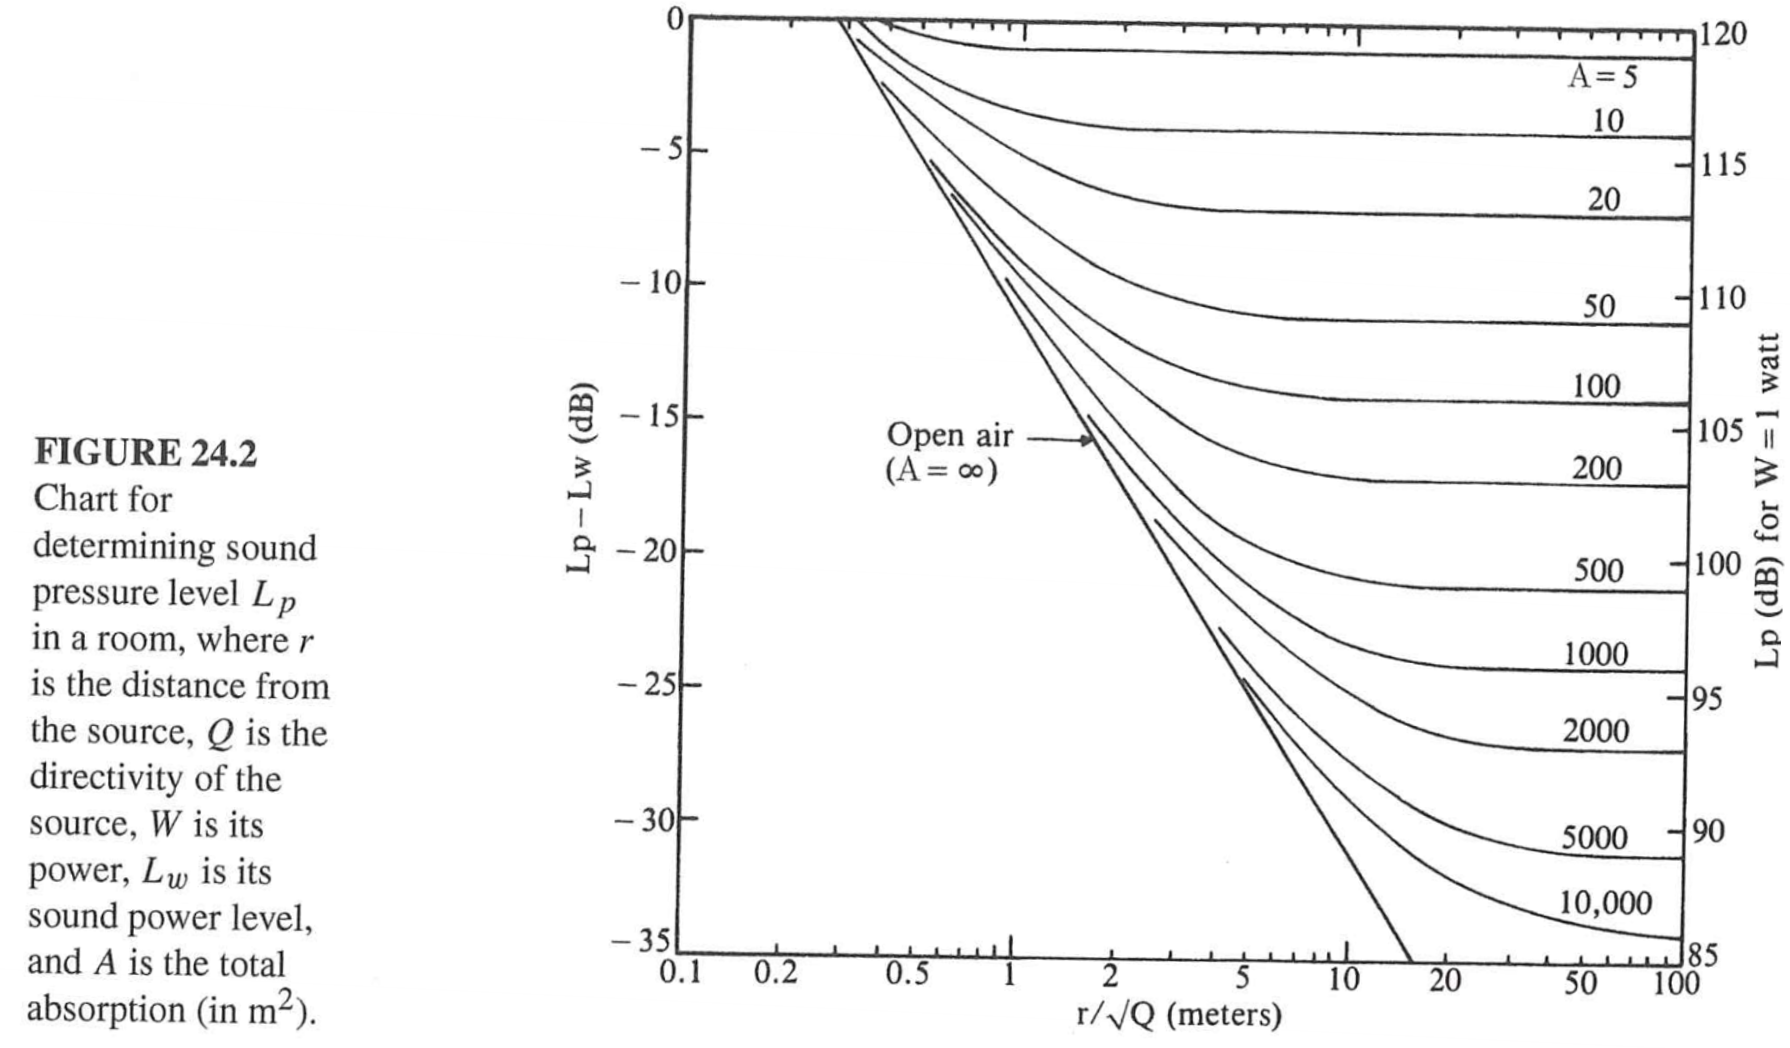
\includegraphics[scale=0.7]{figures/oving2_1.png}
   \caption{Illustration from "Science of Sound", chap 24.}
    \label{fig:nc}
\end{figure}

\end{document}
